\documentclass[
%  master,
%  field=inf,
%  printversion,
  biblatex,
%  language=czech,
%  font=sans,
  glossaries,
  index
]{kidiplom}

\title{Mobilní aplikace pro pracovníky pečovatelské služby}
\title[english]{Mobile application for workers of the day care}
\author{Petr Janiš}
\supervisor{Mgr. Radek Janoštík}
\yearofsubmit{2020}
\annotation{TODO}
\annotation[english]{TODO}
\keywords{TODO; TODO}
\keywords[english]{TODO; TODO}
\thanks{Thanks TODO}
\usepackage{lipsum}
\usepackage{float}

\begin{document}
\maketitle

\section{Úvod}

\newpage

\section{Vývoj mobilních aplikací}
Mobilní aplikace by uživateli měla, co nejjednodušeji a nejrychleji umožnit dosáhnout jeho cíle. Tento fakt je potřeba mít na paměti v průběhu celého procesu vývoje. Je důležité, aby aplikace běžela plynule a měla jednoduché uživatelské rozhraní. U aplikací určených pro širokou veřejnost, je dobrý návrh a provedení UI, faktorem rozhodujícím o jejich úspěšnosti na trhu. Co se týče mobilního softwaru vyvíjeného za účelem korporátního použití, je to otázka finanční náročnosti pro firmu, která se ho rozhodne používat. Jednodušší ovládaní znamená měně potřebného času a prostředků vynaložených na zaškolení zaměstnanců.

Pro plynulý běh aplikace je důležité hned na začátku vývoje přesně určit
 za jakým účelem bude používána. Tato specifikace společně s platformou, 
 na kterou by měl být vývoj cílen, jsou rozhodujícími kriterii při výběru frameworku a způsobu vývoje.

V dnešní době se na trhu s mobilními telefony vyskytují v převážné míře pouze dva operační systémy. Android, který podporuje zařízení od vícero výrobců. A iOS od firmy Apple, který je určen přímo pro hardware od toho výrobce. Ovšem tyto systémy mají spoustu rozdílných verzí. Samotná zařízení mají rozdílné velikosti, funkce a vnitřní komponenty. Tohle je pravě to, co činí vývoj mobilních aplikací složitým a zdůrazňuje důležitost výběru správné metody. Aby bylo možné toto klíčové rozhodnutí udělat správně, je potřeba se seznámit s detaily různých stylů vývoje a frameworky.

\subsection{Nativní vývoj}
Při této metodě je aplikace tvořena odděleně pro každou platformu zvlášť. Stejný kód je tedy potřeba napsat dvakrát v různých programovacích jazycích, použít různá vývojová prostředí a nástroje. Nehledě na to, že Apple neumožňuje vývoj nativních aplikací na jiném operačním systému než MacOS. 

Pokud by tedy výsledný software měl běžet na obou platformách, což je ve většině případů předpokladem, firma by musela mít dva týmy, každý pro jednu část a poskytnout jim rozdílné vybavení. Nejenom, že tímto způsobem bude vývoj trvat dlouho, ale zároveň bude i drahý. Na druhou stranu výsledkem bude snadno udržovatelná a výkonná aplikace umožňující využívat všech funkcí zařízení. Knihovny, které jsou použity spravují samotní vlastníci platforem. Je tedy možné rychle nebo úplně bez zásahu reagovat na nové verze systémů a změny v designu nativních komponent. 

Výsledný produkt je potřeba šířit mezi uživatele. K tomuto účelu slouží takzvaný ''Store'' a každá platforma má svůj vlastní. Obě firmy se snaží vytvořit bezpečné prostředí pro uživatele a kontrolují aplikace sdílené pomocí této služby. Otevřená povaha Androidu ovšem umožňuje mít více než jedno centrální místo pro získání aplikace a proto se snaží řešit část bezpečnostních rizik už na straně kódu a knihoven. Apple je v tomto ohledu daleko přísnější a kontroluje každou aplikaci, která je do App Storu přidána. Někdy trvá i několik dní než prohlásí aplikaci nebo aktualizaci za důvěryhodnou. V tomto procesu se kontroluje hlavně jestli produkt opravdu dělá to, co vydavatel tvrdí v popisu a splňuje všechny bezpečnostní normy. Tyto bezpečností aspekty za vývojáře, do určité míry, je schopno pohlídat nativní vývojové prostředí a kompilátor. Tímto způsobem je tedy možné se vyhnout neschválení aplikace firmou Apple a bezpečnostních nedostatků na jiných platformách. Tento přístup je tedy vhodný pro specifické typy projektů:
\begin{itemize}
	\item Tam kde není potřeba, aby výsledná aplikace běžela na obou platformách.
  	\item Je kladen důraz na výkon aplikace, nebo je to z podstaty požadavků nutnost.
  	\item Hraje velkou roli bezpečnost a není žádoucí používaní knihoven a frameworků třetích stran. 
  	\item Neklade se důraz na rychlost vydaní aplikace na trh a cenu produktu.
 \end{itemize}

\subsubsection{Android}
Aplikace pro Android mohou být napsány pomocí jazyků Kotlin, Java a C++. Nástroj Android SDK zkompiluje kód společně s daty a soubory obsahujícími zdrojové kódy do APK, což je archivní soubor s příponou .apk. APK soubor obsahuje všechny komponenty aplikace a zároveň je to soubor, který zařízení s operačním systémem Android používají k instalaci.
\cite{1}
\textit{(volný překlad)}

K vývoji pro platformu Android je tedy potřeba Android SDK a vhodné vývojové prostředí. Dle dokumentace je doporučovaným vývojovým prostředím Android studio. Velkou výhodou je, že tyto nástroje mohou běžet na jakémkoliv operačním systému.

\subsubsection{iOS}
iOS SDK je balíček nástrojů umožňujících vývoj mobilních aplikací na operační systém iOS. Nástroje umožňují vývojáři přistupovat k různým funkcím a službám iOS zařízení jako jsou hardwarové a softwarové atributy. Obsahuje také iPhone simulátory, které kopírují vzhled a pocit z užívání skutečných zařízení. Aby bylo možné aplikaci testovat a distribuovat ji přes App Store, je potřeba zaplatit vývojářskou licenci. SDK společně s vývojovým prostředím Xcode pomáhá psát aplikace pro platformu iOS za použití oficialně podporovaných  jazyků, kterými jsou Swift a Objective-C. 
\cite{2}
\textit{(volný překlad)}

\subsection{Multiplatformní vývoj}
Umožňuje vývoj na obě platformy současně a v některých případech pro ně používá i identický kód. Každý framework toto umožňuje trochu jiným způsobem. Základní myšlenka je ale taková, že na rozdíl od nativních aplikací, které komunikují přímo s operačním systémem a zařízením, je u multiplatformních aplikací přidána abstraktní mezivrstva neboli nativní obálka. Mezivrstva zaručuje to, že se aplikace pro systém telefonu tváří jako nativní a zároveň umožňuje kódu přístup ke všem periferiím zařízení jako jsou kamera, určovaní polohy, gyroskop atd. Vzhled takto napsaných aplikací bude naprosto totožný s nativní verzí. Tato obálka ovšem zpomaluje chod aplikace, protože každý proces, který vyžaduje komunikaci se systémem přes ní musí projít a mezivrstva jej musí zpracovat. Toto zpomalení je možno považovat za zanedbatelné, pokud není cílem vývoje například hra, aplikace s robustním uživatelským rozhraním nebo s velkým množství rychle vstupujících dat. Celkově tato metoda v porovnaní s klasickým přístupem poskytuje levnější a většinou i rychlejší cestu k vývoji aplikace. 

Na druhou stranu projekt může být vystaven riziku zastavení podpory pro zvolený framework, vrstva navíc znamená prostor pro více bezpečnostních nedostatků a každý vývojář musí být obeznámen s detaily fungování obou platforem. I přesto, že je tímto způsobem možné vyvíjet aplikaci na obě platformy za použití počítače s jakýmkoliv operační systémem, tak pro kompilaci a testování kódu bude v případě iOS nutné použít stroj s macOS. 


\subsubsection{React Native}
React Native je open-source framework, který umožňuje vývoj aplikací pro Android a iOS za použití Reactu a nativních možností platformy. Používá skriptovací jazyk JavaScript, za pomocí kterého se přistupuje k API konkretní platformy. Zároveň popisuje vzhled a chování  uživatelského rozhraní za použití komponent Reactu.
\cite{3}
\textit{(volný překlad)}

Důležitou vlastností je to, že kód je kompilován do nativního jazyku používaného platformou. Velkou výhodou je, že pokud žádná z poskytovaných knihoven neobsahuje danou funkcionalitu, je možné vytvořit modul, v některém z nativních jazyků a zaintegrovat jej do projektu. Za kvalitu framewoku mluví to, že je aktuálně nejpoužívanější ve své kategorii a jsou pomoci něj vytvořeny aplikace jako Facebook a Instagram, které denně používají milióny uživatelů.

\subsubsection{Xamarin}
Xamarin je opět platforma, která umožňuje multiplatformní vývoj, tentokrát ale s rozdílem, že společně s mobilní verzí je možné tvořit i aplikaci pro Windows. Patří do rodiny nástrojů .NET čili kód je psán v programovacích jazycích C\# a F\#. Microsoft využívá už nabitých zkušeností vývojářů s jejich předešlým nástrojem WPF a architekturou Model-View-ViewModel. Většina kódu je sdílená, Microsoft uvádí až 90\% \cite{4}, ale je možné určité části vytvořit speciálně pro jednu platformu. V této části je struktura kódu a volaní systémového API velice podobná nativnímu vývoji, pouze za použití jiného jazyka.
%% MONO

\subsubsection{Capacitor}
Nástroj, který umožňuje spuštění webových aplikací jako nativních. Takto vytvořené aplikace jsou také nazývány jako hybridní. Na rozdíl od React Native se kód tvořený HTML, CSS a JavaScriptem nepřekládá. Namísto toho se uvnitř přidané abstraktní vrstvy otevírá takzvané web view. Web view je v podstatě vestavěný webový prohlížeč, který se stará o běh a zobrazení kódu, lze vidět na obrázku ~\ref{fig:HybridArchitecture}.  

\begin{figure}[H]
  	\centering
 	 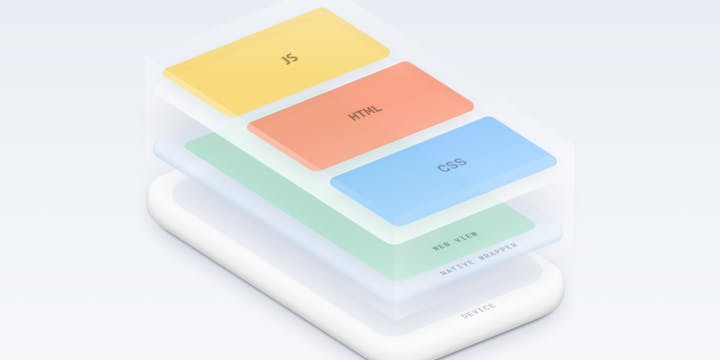
\includegraphics[width=12cm,height=10cm,keepaspectratio]{hybridni_aplikace}
 	 \caption{\cite{5} Architektura hybridních aplikací}
 	 \label{fig:HybridArchitecture}
\end{figure}



Přístup k nativní API je poté zařízen přes pluginy volané z JavaScriptu, které propojují web view s nativní obálkou. Zde už je zpomalení poněkud výraznější a proto se tento způsob doporučuje pouze pro menší až středně velké projekty s nepříliš složitým uživatelským rozhraním, které by potencionálně mohlo na pozadí generovat veliké množství DOM elementů. Možnost vytvořit, z kterékoliv webové aplikace nativní aplikaci je hlavní výhodou, ale tvoří problém s nekonzistentním designem uživatelského rozhraní a nepřipraveností webu pro běh na mobilním zařízení. Z tohoto důvodu je dobré používat tento nástroj v kombinaci s některým z framewoků, které jsou k tomu uzpůsobeny.

\subsection{Progresivní webové aplikace(PWA)}
Jsou webové aplikace plně využívající možností moderních webových prohlížečů. Posouvají tím možnosti jejich funkcionality a pocitu z užívaní na úroveň blížící se nativním a multiplatformním aplikacím. Mohou být ale řazeny mezi ostatní mobilní aplikace? Pokud jako definující vlastnosti mobilních aplikací označíme přístup k periferiím zařízení a systémové API, spuštění i bez přístupu k internetu a nutnosti zapnutí webového prohlížeče, provádění procesů na pozadí. Potom ano.

Prvním stavebním blokem této technologie jsou takzvané service workery. Service worker je skript, který běží na pozadí, odděleně od webové stránky a umožňuje tak funkcionalitu, která nepotřebuje webovou stránku nebo interakci uživatele. \cite{6} \textit{(volný překlad)} Řeší tedy procesy na pozadí a zároveň ukládají kód stažený z webového serveru do aplikační cache a tím umožňují spustit aplikaci bez přístupu k internetu. Na zařízeních používající iOS jsou některé možnosti těchto skriptů omezeny, ale nejedná se o klíčovou funkcionalitu.

Druhou důležitou součástí jsou webové aplikační manifesty. Je to soubor ve formátu JSON, který určuje jak se bude aplikace chovat a vypadat po ''instalaci'' na zařízení. \cite{7} \textit{(volný překlad)} Instalací se v tomto ohledu myslí přidání ikony na domovskou obrazovku zařízení. Po spuštění přes tuto ikonu se sice otevře výchozí webový prohlížeč a v něm teprve stránka, ale o tomto procesu uživatel vůbec neví. Prohlížeč totiž nemá žádnou ze svých běžných nástrojových lišt a aplikace je otevřena přes celou obrazovku zařízení.

Přístup k periferiím zařízení je potom umožněn různou kombinací funkcí prohlížeče, HTML5 a JS. Zde je ovšem oproti nativním a multiplatformním aplikacím výběr omezenější.

\subsection{Backend pro mobilní aplikace}
Většina aplikací se neobejde bez serverové části. Buď z důvodu získání dat nebo komunikace s jinými instancemi aplikace. Server by měl vykonávat většinu výpočetních operací a posílat pouze nezbytně nutná data, aby co nejméně zatěžoval mobilní zařízení. Jako nejlepší postup se tedy může zdát vytvoření vlastní API přímo na míru konkrétní aplikace. Toto řešení zvyšuje výdaje za vývoj i údržbu systému. Zbytečným se stává obzvláště v situacích, kdy by měl server provádět pouze jednoduché operace, jako ověření identity uživatele. Pro projekty této povahy je tedy vhodnější použití cloudových služeb. Tyto služby umožňují vytvoření databázové struktury a na tomto základě vystavení REST API, které může aplikace konzumovat.
\newpage

\section{Výběr technologií}
Ještě před výběrem konkretních technologií a programovacích jazyků jsem se zamýšlel nad způsobem, jak výsledný produkt předat potencionálnímu zákazníkovi. Rozhodnutí nakonec bylo, tento problém kompletně eliminovat, celý systém kontejnerizovat pomocí nástroje Docker, kromě výsledných nativních aplikací, u kterých to postrádá smysl. Při výběru technologií jsem tak nebyl vázán na prostředí, ve kterém systém poběží.

\subsection{Docker}
TODO
 
\subsection{Klientské části}
Základním a nejdůležitějším cílem bylo vytvořit aplikaci, která bude funkční v mobilních zařízeních s operačními systémy Android i iOS a zároveň ve webových prohlížečích. Protože jsem byl na vývoj sám a chtěl jsem vytvořit kvalitní aplikaci, nativní vývoj pro každou platformu s následným vytvořením webové verze nepřipadal v úvahu. Webová aplikace s následným zabalením do nativní obálky je v dané situaci nejvíce vyhovujícím řešením. Jako nástroj pro převod jsem použil výše zmíněný Capacitor. 

Posledním krokem bylo zvolit správný přístup k vývoji webové aplikace. Tradiční způsob tvoření webové stránky za použití HTML, CSS a JavaScriptu by bylo zdlouhavé a potencionálně nebezpečné. Aplikace by očividně obsahovala spoustu kódu v čistém JS, který nemá žádnou kontrolu datových typů, což ve větších projektech může způsobovat chyby, které není lehké odhalit. Další problém by nastal se samotným uživatelským rozhraním. Veškeré UI komponenty by museli být vytvořeny ručně a nebyla by zaručena konzistence se zásadami stylů platformy. Upravovat styl stránky pomocí CSS, tak aby fungovala na zařízeních všech velikostí je sice možné, ale zbytečně náročné. Z těchto důvodů jsem se rozhodl použít framework Angular a platformu Ionic, která je navíc výborně kompatibilní s pluginy Capacitoru.

\subsubsection{Angular}
Angular je platforma a framework pro vývoj jednostránkových klientských aplikací za použití HTML a TypeScriptu. Samotný Angular je napsaný v TypeScriptu. Implementuje základní a volitelné funkce jako množinu TypeScriptových knihoven, které je možné importovat do aplikace. \cite{8} \textit{(volný překlad)} 

Jednostránkové klientské aplikace fungují tak, že při prvním přístupu na stránku se do klientova zařízení stáhnou všechny soubory potřebné k běhu aplikace. Při jakékoliv další akci uživatele se stránkou už se nikdy nepřistupuje na webový server. Tento mechanizmus značně ulehčuje service workeru práci s cachovaním a následným spouštěním aplikace v offline režimu, v případě, že by bylo potřeba z aplikace vytvořit PWA.

TypeScript je nadmnožina skriptovacího jazyku JavaScript a přidává do něj možnost typování proměnných, parametrů a návratových hodnot funkcí. Je to objektově orientovaný jazyk podporující funkcionální paradigma s prvky asynchroního programování. Webové prohlížeče ovšem tento jazyk neumí zpracovat a proto je potřeba provést transpilaci. Transpilace je proces, při kterém se všechny soubory projektu přeloží do souborů s příponou .js, které se navzájem referencují. A dále do index.html souboru, který je kořenem tohoto stromu závislostí.

Základními stavebními bloky jsou komponenty a služby. Komponenty se skládají z náhledů a kódu na pozadí. Náhled je HTML kód, doplněný o takzvané directivy, které umožňují například psát cykly a podmínky jako atributy HTML tagů. Kód na pozadí je vždy třída, obsahující metody a atributy, které je možné referencovat v náhledu. Služby obsahují funkcionalitu, která přímo nesouvisí s náhledy a je možné je do komponent ''injectovat'' jako závislosti. \cite{8} Framework tedy automaticky nabízí podporu návrhového vzoru Dependecy injection a všechny služby jsou typu Singleton. Architektura založená na používaní komponent usnadňuje znovupoužitelnost kódu.

\subsubsection{Ionic}
Platforma, která ulehčuje vývoj webových aplikací cílených na mobilní zařízení. Poskytuje vývojářům množství komponent, které se vzhledově přizpůsobují dle platformy, na které běží. Projekty vytvořené pomocí nástrojů, které platforma nabízí jsou plně responzivní. Ionic rozšiřuje základní knihovnu Angularu o nové stavy životních cyklů komponent a navigační strategii, která umožňuje uchovávat si navigační zásobník instancí naposledy otevřených náhledů. Dohromady je díky nim možné implementovat chování navigačních tabů, na které jsou uživatelé nativních aplikací zvyklí. 

\subsection{Server}
Vzhledem ke zvolené technologii pro aplikaci bylo lepší, co nejvíce zodpovědnosti za operace s daty předat serveru a odlehčit tak zařízením, na kterých poběží. Zároveň jsem chtěl mít plnou kontrolu, nad tím jak serverová část zpracovává data a v jakém formátu je posílá klientovi. Proto jsem se rozhodl kód serveru psát sám a přímo na míru, místo použití cloudových řešení jako Firebase. 

Základem Angularu zvoleného pro tvorbu klientských částí je JavaScript. JS umí automaticky vytvářet objekty a kolekce z JSON souborů. Angular má navíc v základní knihovně velice dobře zpracovanou podporu pro vytváření HTTP požadavků. Jasnou volbou tedy bylo REST API, které funguje na základě protokolu HTTP a standardním formátem pro přenos dat je právě JSON. S přihlédnutí na budoucí rozšíření bylo žádoucí, aby vybraná technologie umožňovala případné rozšíření o gRPC služby založené na protokolu HTTP/2, kvůli plně duplexní komunikaci.

Dalšími faktory při výběru byly: dobrý vestavěný framework pro práci s databází, podpora pro ověřování identity uživatele pomocí JSON Web Tokenů, podpora nástroje Swagger pro dokumentaci, nezávislost na operačním systému a ideálně i vestavěná podpora pro Docker. Konečným výběrem tedy byl ASP .NET Core.

\subsubsection{.NET Core}
.NET Core je open source framework pro operační systémy Windows, Linux a macOS. Je to multiplatformní nástupce .NET Frameworku. Projekt je primárně vyvíjen firmou Microsoft a vydáván pod MIT Licencí. \cite{9} \textit{(volný překlad)} Při práci s .NET Corem jsou používány jazyky C\#, F\# a VisualBasic.

ASP .NET Core slouží k vývoji webových aplikací a služeb s tímto vývojem spojených.
\newpage
\section{Server}
%% uvod

\subsection{Databázový modul}
Prvním krokem při vývoji serverové části bylo vytvoření modulu pro práci s databází. Stavebním blokem pro tento modul je Entity Framework Core. Zároveň jsem do tohoto modulu přidal nástroj, který generuje testovací data a který je možno explicitně spustit ve formě konzolové aplikace.

\subsubsection{Datové třídy}
 U tvorby tříd odrážejících strukturu datového modelu (příklad v kódu~\ref{code:EntityClass}), bylo potřeba zvolit vhodné datové typy, vyřešit jak simulovat relace mezi jednotlivými tabulkami a rozdíl mezi povinnými a nepovinnými parametry:
\begin{itemize}
	\item Název tabulky určuje anotace Table. Kód ~\ref{code:EntityClass} na řádku 1. 
	\item Jako identifikátor jsem zvolil datový typ Guid, který umožňuje přímo identifikovat určitý záznam v databázi.
	\item Atributy s hodnotovými datovými typy jsou označeny jako nullable, pokud nejsou povinné.
	\item K atributům s referenčními datovými typy je přidána anotace Required, pokud jsou povinné, kód ~\ref{code:EntityClass} řádky 4 a 7.
	\item V případě relace 1:N. Pro stranu 1 je simulována kombinací atributu pro uložení cizího klíče a referencí na instanci třídy reprezentující jinou tabulku(navigační atribut), kód ~\ref{code:EntityClass} řádky 10 a 11. Pro stranu N bude navigační atribut kolekce těchto typů.
\end{itemize}

\begin{kicode}{csharp}{code:EntityClass}{Objekt reprezentující databázovou tabulku.}
[Table("User")]
    public class User : EntityBase
    {
        [Required]
        public string LoginName { get; set; }

        [Required]
        public string Password { get; set; }

        public Guid EmployeeId { get; set; }

        public virtual Employee Employee { get; set; }
    }
\end{kicode}

\subsubsection{Db Context}
Datové třídy jsou spojeny ve třídě DbContext, jejíž instance reprezentuje spojení s databází. Na úrovni této třídy je zároveň řešeno, jaký databázový poskytovatel bude použit. Dle toho je potřeba integrovat správnou knihovnu. Připojení k serverům s jiným poskytovatelem je možné libovolně měnit s minimem úsilí. Právě tato třída umožňuje ostatním modulům číst a zapisovat data do databáze. Zodpovědností modulu přistupujícího k datům je předat contextu connection string, díky kterému je možné spojení navázat. V celém projektu je pro práci s daty použit dotazovací jazyk LINQ s rozšířením, které umožňuje dotazování za pomocí lamba výrazů.

Balíček EFCore Tool umožňuje za použití příkazové řádky vytvářet Migrace. Migrace je automaticky vygenerovaný kód, lišící se dle momentálně použitého databázového poskytovatele, popisující strukturu databáze danou DbContextem. Tento kód poté může být použit pro tvorbu oné struktury do aktuálně připojené instance databáze. Tento přístup se nazývá Code first.

Pro načítaní hodnot do navigačních atributů objektů představující záznamy v databázi, je použita metoda Lazy loading. Na rozdíl od ostatních možných přístupů zaručuje, že data budou načtena vždy, až to opravdu bude nutné a současně o to není potřeba explicitně žádat. Toho efektu jsem docílil označením všech klíčových atributů jako virtuálních, což umožňuje, aby se na na jejich místě vytvořili proxy objekty.

\subsection{Struktura API}
TODO úvod
\begin{figure}[H]
  	\centering
 	 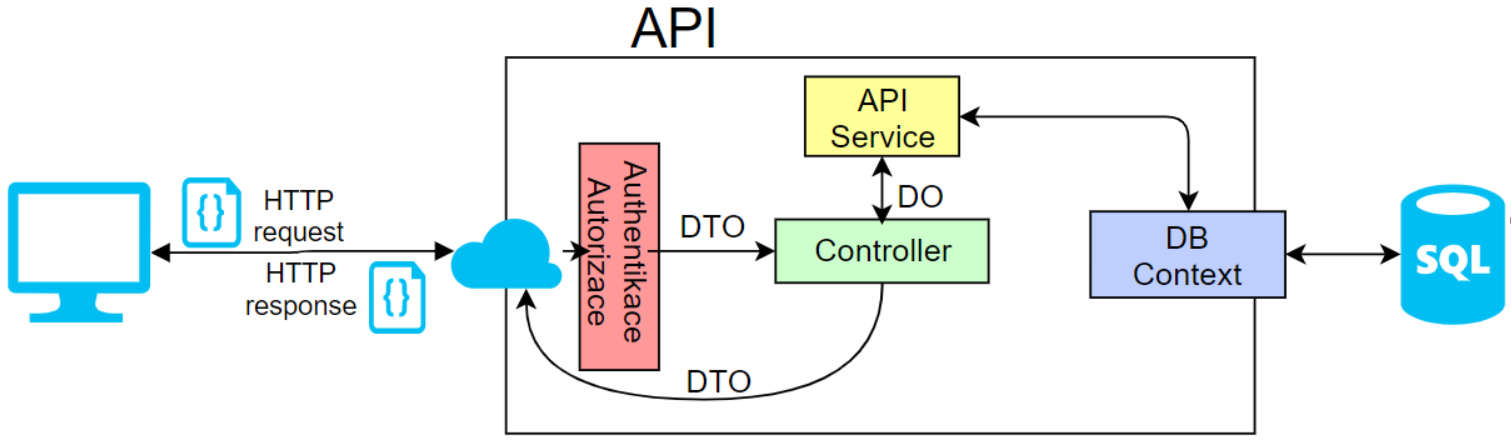
\includegraphics[width=14cm,height=10cm,keepaspectratio]{API_Diagram}
 	 \caption{Diagram struktury API}
 	 \label{fig:ApiStructure}
\end{figure}

\subsubsection{API controllery}
Pomocí controllerů se definuje celá struktura API. Obsahují metody, které jsou volány pomoci HTTP požadavků. 

\begin{kicode}{csharp}{code:Controller}{Ukázka kódu controlleru}
	[Route("api/[controller]")]
	[ApiController]
	[Authorize]
    public class EmployeeController : DssBaseController
    {
        private readonly IEmployeeApiService _employeeApiService;

        public EmployeeController(IEmployeeApiService employeeApiService)
        {
            _employeeApiService = employeeApiService;
        }

        [HttpPost]
        [Authorize(Roles = "Manager")]
        public EmployeeDetailDTO CreateEmployee(EmployeeDetailDTO dto)
        {
            var employee = MapDetailDtoToEmployee(dto);
            var createdEmployee = _employeeApiService.CreateEmployee(employee);
            var createdDto = MapEmployeeToDetailDto(createdEmployee);

            return createdDto;
        }
        ...
\end{kicode}

Proces životního cyklu požadavku z pohledu API začíná ve chvíli, kdy je přijat nějakým z endpointů. To jaký controller by ho měl zpracovat, záleží na použité směrovací strategii a URI, na kterou byl zaslán. S použitím výchozího směrování, jako jsem použil já, a definice cesty v anotaci jako v kódu ~\ref{code:Controller} na řádeku 1 by controller v ukázce ~\ref{code:Controller} obsluhoval všechny požadavky na  adrese: \textit{[základní\_adresa]}/employee/... Jestli je potřeba, aby byl požadavek opatřen platným tokenem určuje anotace Authorize. Řádkem 3 v kódu ~\ref{code:Controller} je tedy dáno, že všechny  požadavky, které tímto controllerem budou obslouženy, musí být takto zabezpečeny.   

HTTP metod je dohromady 8, ale v projektu jsou použity pouze 4 z nich a při jejich použití jsem se držet konvencí: 
\begin{itemize}
	\item \textbf{GET} - je používána pro získání informací ze serveru. Měla by být používána pouze pro získání dat a neměla by na data mít žádný jiný efekt. \cite{10} \textit{(volný překlad)}
	\item \textbf{POST} - používá se pro zaslání dat na server.\cite{10} \textit{(volný překlad)}
	\item \textbf{PUT} - Nahrazuje všechny aktuální reprezentace daného zdroje nahrávaným  obsahem.\cite{10} \textit{(volný překlad)}
	\item \textbf{DELETE} - Smaže všechny aktuální výskyty zdroje uvedeného v URI.\cite{10} \textit{(volný překlad)}
\end{itemize}
Metoda \textit{CreateEmployee} bude díky anotaci na řádku 13 data ukládat a reagovat pouze na POST requesty. 

Posledním aspektem, který je potřeba zmínit, je rozdělení rolí. V systému jsou role dvě: pracovník pečovatelské služby a vedoucí pracovník. Každá role má jiná práva a tím pádem může přistupovat k různým endpointům a získávat tak odlišná data. Pracovník pečovatelské služby je základní role s minimálními oprávněními pro vstup do systému, proto metody konzumovány tímto typem účtů není potřeba explicitně kontrolovat. Při přihlášení se do tokenu ukládá informace(claim - viz ~\ref{sec:security}) o této roli a ta je kontrolována, pokud je metoda označena stejně jako na řádku 14.

Framework automaticky serializuje a deserializuje objekty z a do formátu JSON. Pro vývojáře je tento proces naprosto transparentní a muže rovnou pracovat s objekty, jak jsou definovány v kódu. Z důvodu bezpečnosti, znovupoužitelnosti a možné budoucí rozšiřitelnosti kódu jsem se pro práci s DTO rozhodl použít strategii řídící se následujícími pravidly: 
\begin{itemize}
	\item Návratový typ metody controlleru je vždy DTO obsahující jen ty nejnutnější údaje.
	\item DTO objekty existují pouze v rozsahu controlleru(předchází problému kruhových závislostí).
\end{itemize} 
Lze pozorovat, že metoda na řádcích 15-22 se tohoto principu drží. Na ~\ref{fig:ApiStructure} je toto demonstrováno mezi conrollerem a API službou, mezi kterými se posílají pouze Domain Objects.

\subsubsection{API služby}
Všechny operace s databází jsou striktně prováděny pouze v této skupině tříd. Správnost databázových dotazů je totiž jediným místem, kde může dojít k sémantickým chybám. Tyto třídy proto implementují rozhraní, obsahující všechny jejich veřejné metody, což činí případné Mockování v následném testování možným. Navíc díky dodržováni pravidel o DTO mohou být kdykoliv v budoucnu využity znovu v jiném modulu. 

\subsubsection{DI a propagace konfigurace}
Framework má zabudovanou automatickou podporu pro návrhový vzor Dependecy Injection(DI). Toho jsem využil pro distribuci DbContextu do API služeb a ty zase do controllerů. Výsledek procesu je vidět v kódu ~\ref{code:Controller} řádcích 6-11. Controller závisí na \textit{EmployeeApiService}, která je reprezentována svým rozhraním.  Při volání tohoto konstruktoru DI kontejner automaticky poskytne její instanci jako parametr.

ASP .NET Core má komplexní systém možností konfigurace, který zvládne konzumovat konfiguraci z mnoha různých zdrojů najednou, upřednostnit parametry s větší prioritou a následně je sloučit. Tohoto je využito například při nastavování proměnných prostředí při spouštění Docker kontejneru.

\subsubsection{Zabezpečení}
\label{sec:security}
Všechny požadavky musí v hlavičce obsahovat platný token, jinak je API odmítne obsloužit. Tyto Json Web Tokeny vystavuje jediný nezabezpečený endpoint, který přijímá jako parametry jméno a heslo uživatele. Hesla jsou v databázi uložena v hashované podobě, proto je nutno udělat to stejné a převést heslo pomocí hashovací funkce MD5. Pokud ověření proběhne v pořádku, je vytvořen nový token, který je podepsán soukromým klíčem a jsou do něj zakódovány informace jako jméno uživatele, datum a čas expirace, kdo je konzument, vydavatel tokenu a role. Tyto informace se nazývají claimy a je možné je z tokenu kdykoliv vyčíst. Jediná informace, která zaručuje bezpečnost, je právě soukromý klíč, kterým se ověřuje, že přijatý token byl vystaven právě touto API.

\subsubsection{Swagger a automatická dokumentace}
Pro účely dokumentace API jsem použil nástroj Swagger, který automaticky zpracuje její strukturu a poskytne ji v podobě uživatelského rozhraní a JSON souboru. V produkci je žádoucí tuto funkci vypnout nebo zabezpečit ověřením identity.

\begin{figure}[H]
  	\centering
 	 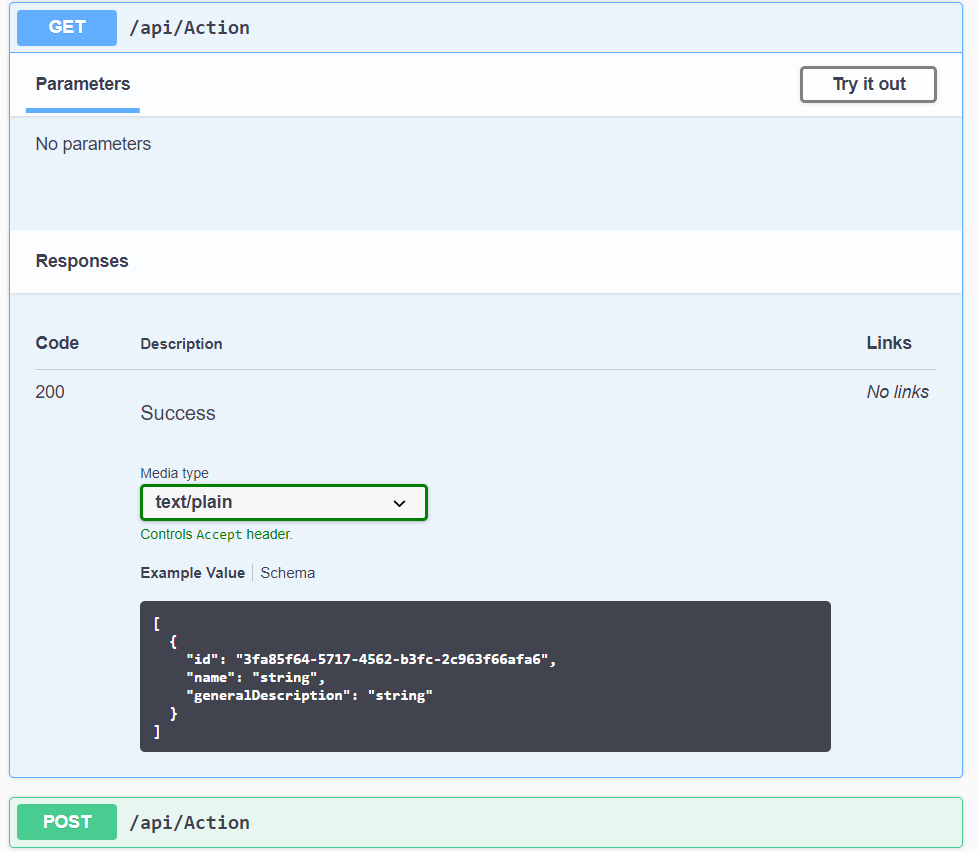
\includegraphics[width=14cm,height=10cm,keepaspectratio]{Swagger_UI}
 	 \caption{Ukázka grafické dokumentace pomocí nástroje Swagger}
\end{figure}

\subsubsection{Generování akcí}
\label{sec:security}
Dle datového modelu(ref. dat model) a jeho popisu v(ref uvod) je vidět, že jednotlivé akce, které pracovníci plní vycházejí z pevně daného rozvrhu. Tyto akce nejsou v databázi uložené všechny a ani být nemohou, protože individuální plán může mít libovolné datum expirace a dat by tedy bylo potencionálně velké množství. Proto jsem se rozhodl akce generovat postupně v době potřeby. Na straně serveru jsem vytvořil patřičnou funkcionalitu a zpřístupnil ji jako API endpoint pro jehož volání je nutná managerská role. Díky tomuto je možné akce generovat automaticky. Automatizovaný mechanizmus jsem neimplementoval, protože je úzce spjat s prostředím na kterém by systém běžel i přesto, že jsem použil Docker. Pro prostředí se systémem Windows by bylo vhodné použít například WCF službu \cite{11}. U cloudových řešení záleží na službách nabízených poskytovatelem. Akce je možné generovat kdykoliv v rámci webové aplikace pro vedoucí pracovníky na období dalšího měsíce.

\subsection{Testování částí}
Testování částí je úroveň testování softwaru, kde jsou testovány individuální komponenty nebo části. Smyslem je ověřit, zdali se každá část chová, jak byla navržena. Část je nejmenší testovatelná jednotka jakéhokoliv softwaru.\cite{12} \textit{(volný překlad)}

Testoval jsem metody API služeb, které provádí složitější databázové dotazy a operace nad těmito daty. Všechny tyto metody používají DbContext pro přístup do databáze. Tento přístup bylo potřeba nahradit testovací instancí databáze, která bude bude na začátku každého testu obsahovat prázdnou strukturu tabulek a po jeho skončení přestane existovat. Pro dosažení tohoto efektu byl DbContext konfigurován pro používání databáze v paměti. Každý test se skládá z těchto stavů: 
\begin{itemize}
	\item \textbf{Arrange} - připraví strukturu dat, tak aby testovala přesnou funkcionalitu testované části.
	\item \textbf{Act} - spustí kód testované části.
	\item \textbf{Assert} - porovnává vrácené výsledky s očekávanými výsledky, pokud se liší, vyvolá chybu.
\end{itemize}

\newpage

\section{Klientské části}
TODO úvod

\subsection{Multiplatformní aplikace}
?úvod?

\subsubsection{Komunikace se serverem}
Díky integraci automatické dokumentace v serverové části jsem získal popis struktury API jako soubor ve formátu JSON. V kombinaci s nástrojem Swagger codegen jsem soubor použil pro vygenerování celého modulu pro komunikaci se serverem. Šablonu, pomocí které se jednotlivé služby generují, bylo potřeba upravit, aby k jednotlivým dotazům do hlavičky přidával token z lokálního úložiště a ty byly tak z pohledu serveru autorizované. Pokud požadavek skončil chybou, je o tom uživatel patřičně informován v podobě notifikace nebo návratem na přihlašovací obrazovku dle povahy chyby.

Problém představoval převod časových údajů z formátu ISO 8601 do datového typu datum v JavaScriptu. ISO 8601 je standardem pro reprezentaci časových údajů ve formátu JSON, který je používán pro přenos dat mezi klientem a serverem. Tento formát na rozdíl od datového typu není závislí na časové zóně. Z tohoto důvodu byl přidán HTTP interceptor, který projde data každého požadavku a odpovědi a upraví v nich data, tak aby jejich hodnota byla korektní dle časové zóny klienta, což ve výsledku ovlivňuje i správnost záznamů v databázi.

\subsubsection{Klientská cache}
HTTP požadavek na API může být časově náročná operace. Proto jsem se rozhodl, při zapínání aplikace načíst a zpracovat nejčastěji používaná data a následně se na ně na všech stránkách pouze odkazovat. Konkrétně jde o data klientů. 

Je důležité zmínit, že jsou načítaní pouze klienti, kteří jsou přihlášenému zaměstnanci přiřazeni pomocí individuálního plánu(ref. data model). Zaměstnanec by totiž neměl být schopen zobrazovat osobní data klientů o které se nestará. Jedinou výjimkou je pokud je zaměstnanci přiřazena jednoúčelová registrovaná akce, poté se zobrazí jen ty nejnutnější informace, které potřebuje ke splnění této akce.

Při tomto načítání se kontroluje, v jakém stavu jsou údaje o klientově adrese. Systém totiž umožňuje uložení bydliště, buď pouze jako souřadnice zeměpisné šířky a délky nebo jako objekt popisující adresu v řetězcích. V různých místech aplikace jsou potřeba oba údaje, proto je případné chybějící udaje třeba doplnit. Za tímto účelem je použita Google Maps Geocoding API. 

Zde se poprvé zjišťuje i poloha zařízení. Ve webových prohlížečích je použita standardní HTML Geolokační API a v případě nativní verze geolokační plugin, který čte data z GPS telefonu a internetového připojení pro větší přesnost. Z tohoto důvodu je uživatel při prvním spuštění požádán o oprávnění k určování lokace zařízení.

V objektu obsahujícím data o klientovi je současně uložena aktuální vzdálenost jeho bydliště od zařízení a výpočet této informace je také součástí procesu načítaní. Přišlo mi zbytečné pro tuto operaci opět používat Google API. V tuto chvíli už je zaručeno, že jsou údaje o zeměpisných souřadnicích adresy a zařízení přítomny a je tak možné použít výpočet pomocí Haversínovy rovnice. Haversínova rovnice (ref. ronice 1) určuje vzdálenost mezi dvěma body ležícími na povrchu koule zadanými zeměpisnou šířkou a délkou.\cite{13} \textit{(volný překlad)} TODO rovnice
$$\left\{\frac{x^2}{y^3}\right\}$$
 Tento výpočet se spouští každých 60 vteřin a aktualizuje, tak informace o vzdálenosti v celé aplikaci.

\subsubsection{Přihlašovací obrazovka}
Po spuštění aplikace je uživatel přesměrován na přihlašovací obrazovku. Uživatel se musí ověřit vůči serveru přihlašovacím jménem a heslem. Aplikace pošle požadavek na na přihlašovací endpoint (viz. sekce ~\ref{sec:security}). Pokud jsou údaje správné uloží si vrácený token do lokálního úložiště prohlížeče a přesměruje uživatele na obrazovku s rozvrhem akcí. V opačném případě uvědomí uživatele, že jsou přihlašovací údaje neplatné.
  
Přesměrovaní na přihlašovací obrazovku nemusí být nutností při každém spuštění aplikace. Před samotným přesměrováním se kontroluje, jestli je v lokálním úložišti uložený token. Prvním požadavkem na server je validována platnost tokenu. Pokud je tedy token validní není potřeba uživatele znovu obtěžovat s přihlašovacím procesem.

\subsubsection{Rozvrh akcí}
Základní obrazovka reprezentující úkony, které by měl přihlášený pracovník provádět nebo už provedl pro konkrétního klienta, lze vidět na obrázku ~\ref{fig:schedule_screen}. Výchozí nastavení obrazovky je takové, že ve vrchním panelu je aktuální datum, reprezentující od kdy budou data zobrazována. 

\begin{figure}[H]
  	\centering
 	 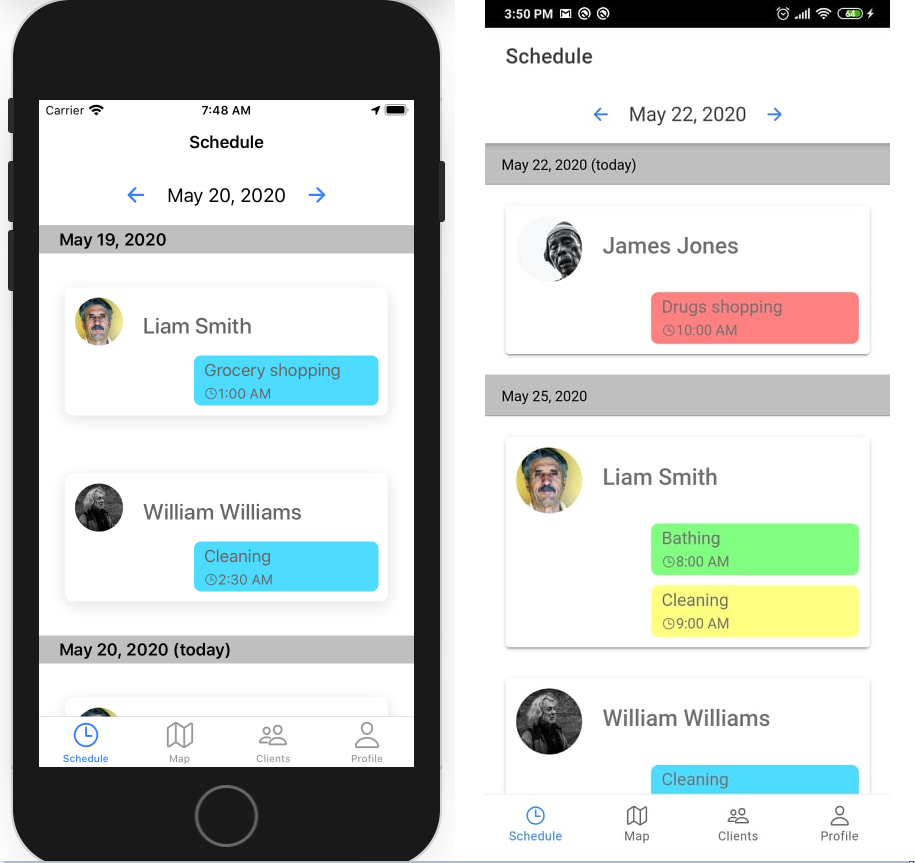
\includegraphics[width=14cm,height=14cm,keepaspectratio]{schedule_screen}
 	 \caption{Obrazovka s rozvrhem akcí(iOS- vlevo, Android)}
 	 \label{fig:schedule_screen}
\end{figure}

Data jsou načítána po dávkách deseti akcí, aby se předešlo dlouhému čekání na odpověď serveru a následného vykreslení. Při pohybu směrem dolů, jsou načítána další data a tento proces je signalizován animací naspodu obrazovky, která je vidět pokud se uživatel nachází za koncem vykreslených dat.

Jednotlivé akce(v kontextu systému jsou nazvány jako registrované akce !ref datovy model!) se mohou nacházet ve čtyřech stavech. Zelený stav znamená, že akce byla dokončena a existují pro ní časové údaje o jejím začátku a konci. Aktuálně probíhající akce jsou značeny žlutě. Pokud z jakýchkoliv důvodu nebyl pracovník úkol schopen splnit nebo byl předem zrušen například samotným klientem je červený. Všechny ostatní jsou modré. Po kliku na akci bude uživatel přesměrován do modálního okna reprezentujícího její detail(viz. sekce ~\ref{sec:actionDetail}).

V případě, že je přihlášený uživatel vedoucí pracovník, kterému systém neumožňuje přiřadit klienty akce na úrovni individuálních plánu ani jednotlivých jednoúčelových akcí. Nebude obrazovka obsahovat žádná data, pouze hlášku upozorňující na absenci akcí v databázi.

\begin{figure}[H]
  	\centering
 	 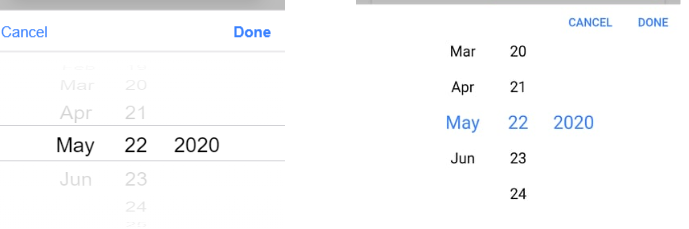
\includegraphics[width=14cm,height=14cm,keepaspectratio]{datepicker}
 	 \caption{Komponenta pro výběr data(iOS-vlevo, Android)}
 	 \label{fig:datepicker}
\end{figure}

Pro prohlížení historických dat nebo rychlejší přesun mezi daty slouží datumový filtr v horní části obrazovky. Tento filtr je možné ovládat buď pomocí šipek, které posunou datum o jeden den nebo výběrem data z komponenty(obrázek ~\ref{fig:datepicker}), kterou lze otevřít kliknutím na datum. Data která je možno vybrat oběma způsoby jsou omezena plánovaným datem první a poslední akce přiřazené přihlášenému zaměstnanci. Na této komponentě je zároveň vidět rozdíl v jejím stylu zobrazení na odlišných platformách, tak aby více zapadala do celkového designu platformy. Styly mnou nebyly v samotném kódu aplikace jakkoliv upravovány. 

\subsubsection{Detail akce}
\label{sec:actionDetail}
Modální okno s detailem akce(obrázek ~\ref{fig:actionDetail}) slouží pro podání detailních informací o akci pracovníkovi pečovatelské služby a evidenci jeho práce.

\begin{figure}[H]
  	\centering
 	 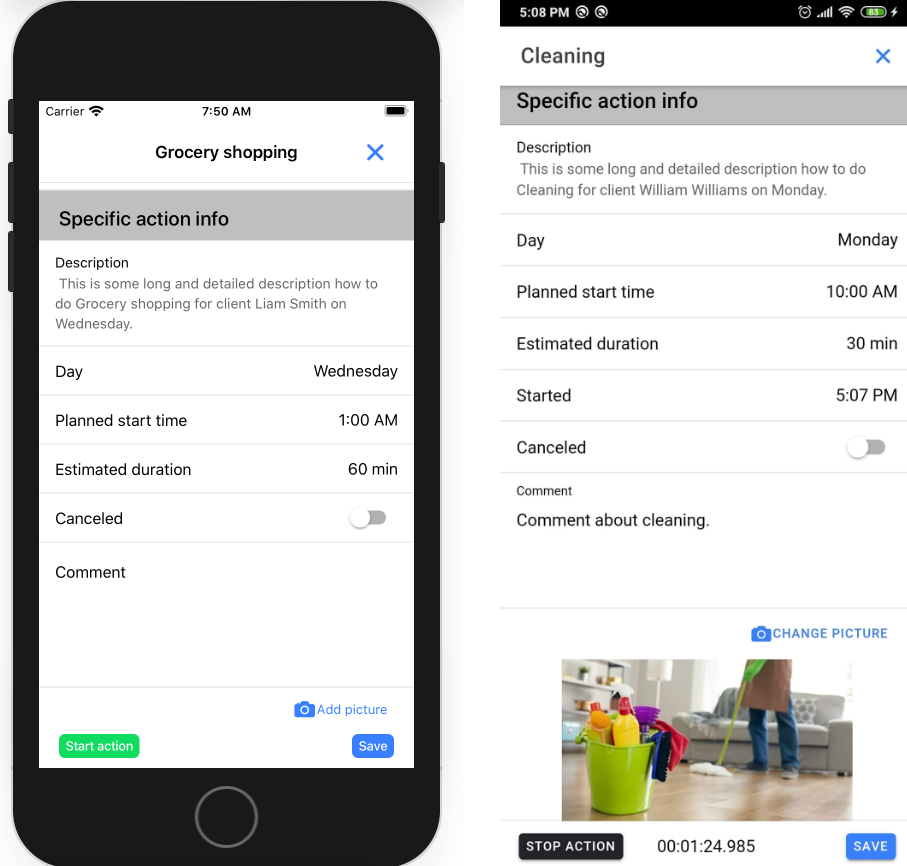
\includegraphics[width=14cm,height=14cm,keepaspectratio]{actionDetail}
 	 \caption{Modální okno s detailem akce(iOS-vlevo, Android)}
 	 \label{fig:actionDetail}
\end{figure}

Každá registrovaná akce je založena na akci všeobecné, která má svůj pracovní postup a ten je zobrazován jako první informace v tomto okně. S tímto postupem musí být pracovníci obeznámeni a zde slouží pouze jako upomínka. Opravdu důležitou informací je specifický popis akce, který se může lišit pro každého klienta a dokonce i podle dne ve kterém je akce vykonávána.

Pro účely fakturace a celkově sledování pracovníku slouží stopovaní trvání akce. Po stisknutí tlačítka pro zahájení akce se spustí stopky a aktuální čas je uložen do databáze. Aplikaci nebo zařízení je tedy možné vypnout a čas na stopkách po návratu zůstane validní. Po zastavení je akce označena za dokončenou.

Akci je možné zrušit pomocí přepínače a uživatel je upozorněn, že je nutno vyplnit komentář a udat tak důvod proč úkon nemohl být proveden. Poslední funkcí tohoto okna je možnost přidání obrázku k akci. Tyto informace na rozdíl od stopování času musí být explicitně uloženy pomocí tlačítka. Způsob přidání obrázku záleží jestli je aplikace spuštěna jako webová nebo nativní verze. Ve webové verzi je výběr fotky umožněn přes HTML input typu soubor, který akceptuje pouze obrázky. V případě nativní verze se otevře výběrové menu ve kterém může uživatel zvolit, jestli si přeje obrázek vyfotit, nebo vybrat z galerie. 

\subsubsection{Mapa s klienty}
Obrazovka s mapou ukazující jednotlivé klienty a aktuální polohou zařízení slouží pro rychlou orientaci (obrázek ~\ref{fig:mapClients}) při dojíždění za klienty. Pro korektní běh všech funkcí musí být povoleno sledovaní lokace zařízení a v případě nativní verze i zapnutá lokalizace telefonu. Pro zobrazení mapy jsem použil komponentu založenou na standardní Google mapě určenou pro použití ve webových stránkách, která pouze poskytuje rozhraní pro lepší manipulaci v rámci Angularu. Vzhled ukazatelů klientů a aktuální polohy jsou vytvořené pomocí HTML a CSS a vložené do mapy na určité zeměpisné souřadnice.

\begin{figure}[H]
  	\centering
 	 
\includegraphics[width=14cm,height=14cm,keepaspectratio]{map}
 	 \caption{Mapa s klienty(iOS-vlevo, Android)}
 	 \label{fig:mapClients}
\end{figure}

Výchozí nastavení filtru zobrazených klientů je takové, že zobrazí pouze ty klienty u kterých má aktuální den přihlášený uživatel naplánované a nezrušené akce. Je zde možné vidět i klienty o které se zaměstnanec pravidelně nestará, ale pouze za předpokladu, že byla vedoucím pracovníkem vytvořena jednoúčelová akce. Tento filtr je možné ovládat pomocí přepínače v otevíracím menu v pravém horním rohu. Po kliknutí na klienta se zobrazí detail, který obsahuje kromě základních údajů o klientovi a jeho adresy i nejbližší naplánovanou akci. 

V případě, že je filtr nataven na zobrazení všech klientů jsou na mapě zobrazení všichni pravidelní klienti. Zde je hledání nejbližší akce poněkud složitější, protože může nastat případ, kdy není akce ještě není vygenerována z rozvrhu. Na straně serveru je z tohoto důvodu mechanizmus, který najde nejbližší akci dle rozvrhu a simuluje generování patřičné akce. Pro aplikaci je tato akce naprosto transparentní a dostane stejná data jako by akce už existovala. Toto je možné pouze v případě zobrazení v detailu na mapě, kde jsou data o akci určena pouze pro čtení a ne pro úpravu jako je to v případě rozvrhu.

Menu obsahující ovládání filtru obsahuje i výčet klientů ve vzdálenosti jednoho kilometru od zařízení. Společně s jejich jménem je zobrazena i vzdálenost od zařízení v metrech. Jejich počet signalizuje podbarvené číslo vedle ikony menu.

\begin{figure}[H]
  	\centering
 	 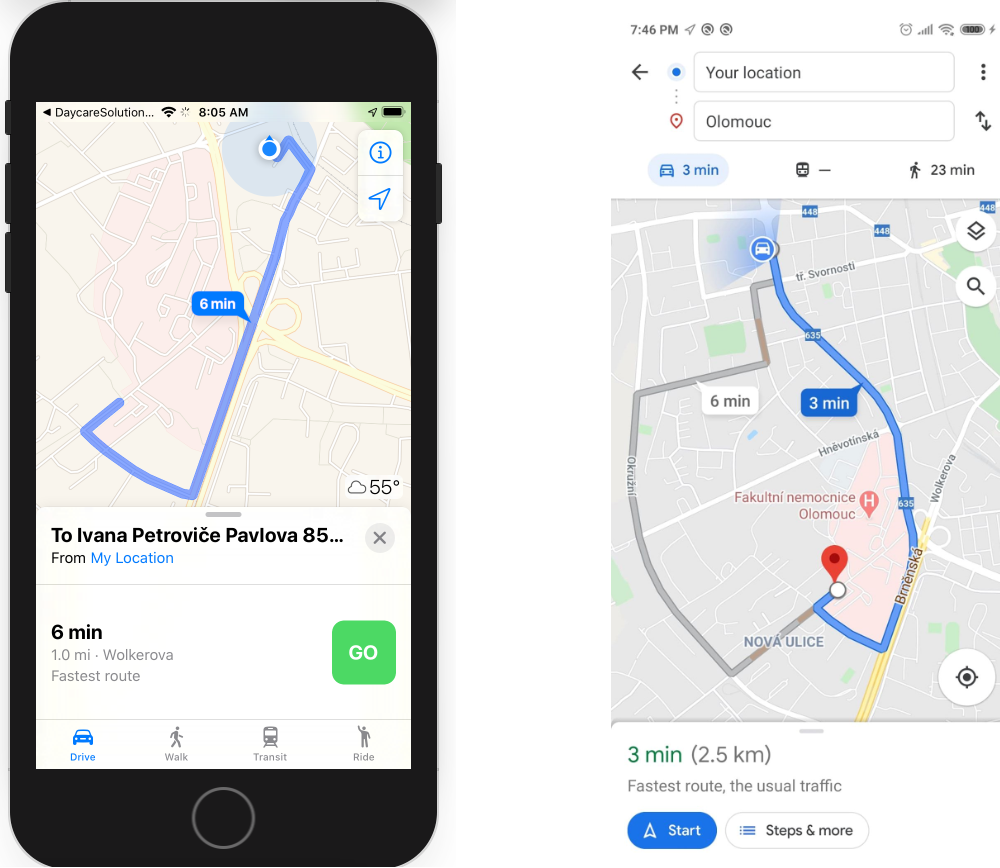
\includegraphics[width=14cm,height=14cm,keepaspectratio]{external_navig}
 	 \caption{Navigace v externí aplikaci(iOS-vlevo, Android)}
 	 \label{fig:externalNavig}
\end{figure}

Ikona navigace v pravém horním rohu detailu klienta umožňuje přesměrování do externí aplikace určené pro navigaci. Pokud je na zařízení nainstalována více než jedna aplikace tohoto charakteru zobrazí se okno s výběrem. Data o klientově adrese jsou automaticky předána externí aplikaci. Na obrázku ~\ref{fig:externalNavig} je ukázka výchozí mapové aplikace pro obě platformy otevřené přes tuto funkcionalitu.

\subsubsection{Informace o klientech}
Úvodní obrazovka sekce o klientech poskytuje přehled všech pravidelných klientů. V případě, že je přihlášen vedoucí pracovník jsou zde zobrazeni všichni klienti, uložení v systému. Kliknutí na kartu s klientem zobrazí přesměrování na detail klienta obsahující všechny jeho informace(obrázek ~\ref{fig:clientDetail}).

\begin{figure}[H]
  	\centering
 	 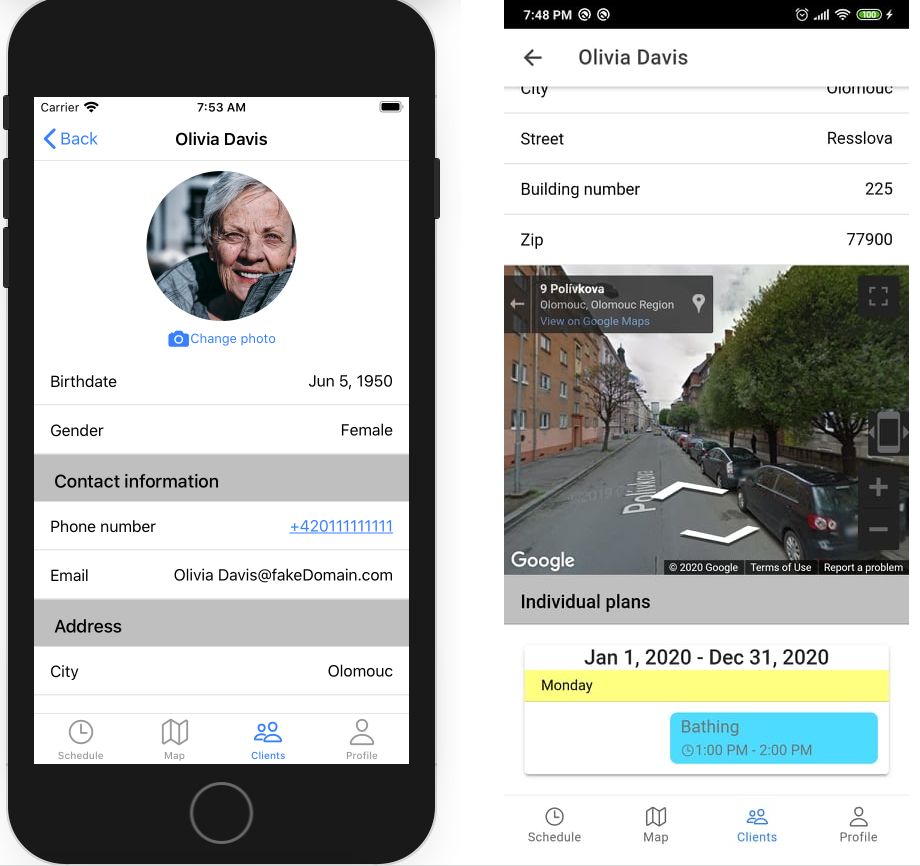
\includegraphics[width=14cm,height=14cm,keepaspectratio]{client_detail}
 	 \caption{Obrazovka s detailem klienta(iOS-vlevo, Android)}
 	 \label{fig:clientDetail}
\end{figure}

Jedinou upravitelnou informací na detailu je foto klienta. Klient má pouze jednoho klíčového pracovníka a tím pádem je tato fotka nejvíce relevantní pro zaměstnance, který má na tuto kartu přístup. Změnu jakýchkoliv osobních údajů by měl obstarávat vedoucí pracovník. 

Při kliknutí na telefonní číslo v nativní aplikaci je uživatel přesměrován do výchozí aplikace pro volání s předvyplněným číslem. Ve webovém prohlížeči na počítači je uživatel dotázán jakým programem si přeje tuto událost obsloužit a v případně prohlížeče Google Chrome je možné tuto informaci poslat do mobilu, který je propojen s uživatelským účtem v prohlížeči.

Detail mimo jiné obsahuje pravidelný rozvrh akcí rozdělený podle jednotlivých individuálních plánů a mapu s ukazatelem na bydliště klienta a možnosti prohlížení pomocí Google Street View.

\subsubsection{Úprava pro velké obrazovky}
Celý styl aplikace a použité komponenty byly původně cíleny pro použití na mobilním zařízení, proto bylo potřeba udělat pár kosmetických úprav, které jsou vidět na obrázku ~\ref{fig:bigScreen}. 

\begin{figure}[H]
  	\centering
 	 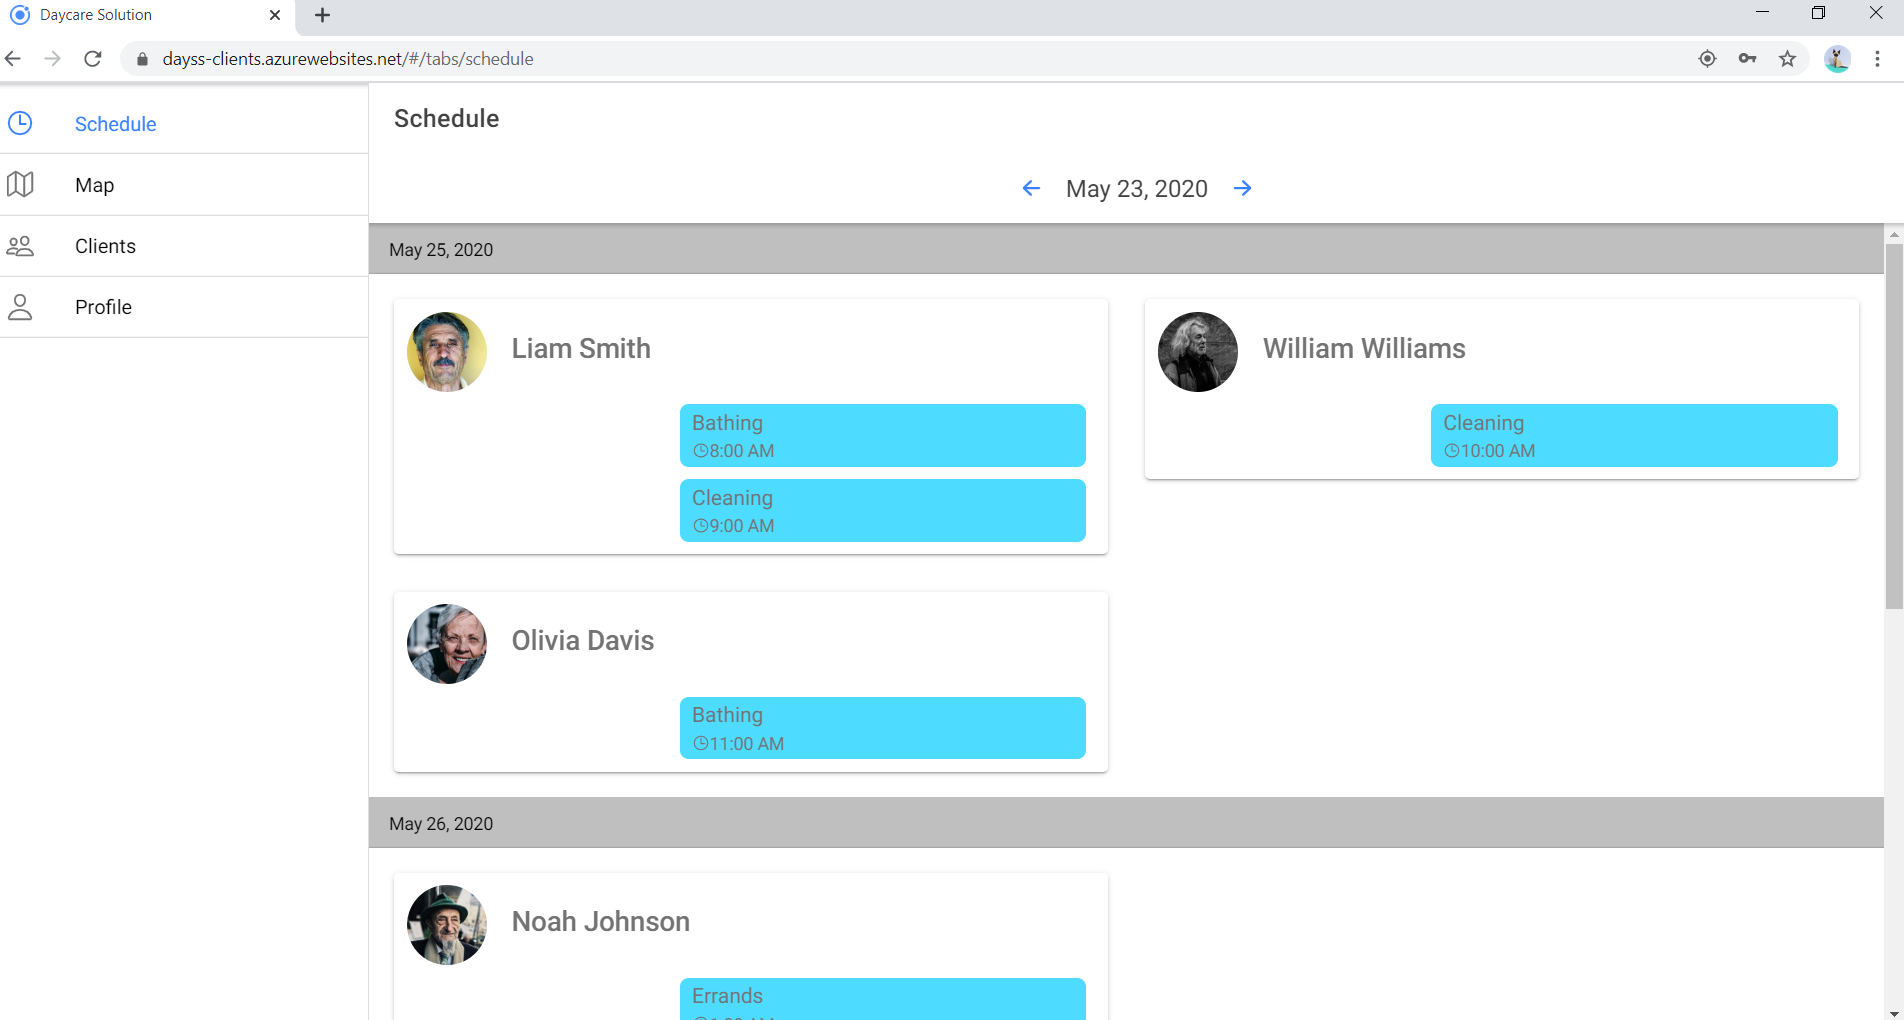
\includegraphics[width=14cm,height=14cm,keepaspectratio]{big_screen}
 	 \caption{Ukázka úprav pro velké obrazovky}
 	 \label{fig:bigScreen}
\end{figure}

Menu v levé části obrazovky nahradilo navigační ''taby'', které nejsou pro použití na velkých monitorech příliš vhodné. Položky menu si ale zachovávají funkcionalitu navigačního zásobníku, která je použita v sekci s klienty. Na všechny stránky s reprezentací dat pod sebou jsem použil grid, který automaticky mění počet položek v řádku z jedné na více podle toho jaké velikosti je okno prohlížeče.

\subsection{Managerská webová aplikace}
%% uvod
%% kalendar a drag and drop

\newpage


\begin{thebibliography}{9}
    \bibitem{1} \url{https://developer.android.com/guide/components/fundamentals}
    \bibitem{2} \url{https://en.wikipedia.org/wiki/IOS\_SDK}
    \bibitem{3} \url{https://reactnative.dev/docs/intro-react-native-components}
    \bibitem{4} \url{https://docs.microsoft.com/en-us/xamarin/get-started/what-is-xamarin}
    \bibitem{5} \url{https://ionicframework.com/resources/articles/what-is-hybrid-app-development}
    \bibitem{6} \url{https://developers.google.com/web/fundamentals/primers/service-workers\#what\_is\_a\_service\_worker}
    \bibitem{7} \url{https://web.dev/add-manifest/}
    \bibitem{8} \url{https://angular.io/guide/architecture}
    \bibitem{9} \url{https://en.wikipedia.org/wiki/.NET\_Core}
    \bibitem{10} \url{https://www.tutorialspoint.com/http/http\_methods.htm}
    \bibitem{11} \url{https://docs.microsoft.com/cs-cz/dotnet/framework/wcf/how-to-host-a-wcf-service-in-a-managed-application}
    \bibitem{12} \url{http://softwaretestingfundamentals.com/unit-testing/}
    \bibitem{13} \url{https://en.wikipedia.org/wiki/Haversine\_formula}
\end{thebibliography}


\newpage
\section{Obsah přiloženého CD/DVD} \label{sec:ObsahCD}
\end{document}
